\documentclass[letterpaper,twocolumn,10pt]{article}
\usepackage{usenix,epsfig,endnotes}
\usepackage [utf8x]{inputenc}
\usepackage{graphicx}
\usepackage{sidecap}
\usepackage{float}
\usepackage{natbib,hyperref}
\usepackage{indentfirst}
\usepackage[T1]{fontenc} 
\usepackage{amsfonts}
\usepackage{tabularx}
\usepackage{listings}
\usepackage{color}
\usepackage{xcolor}
\usepackage{caption}
\usepackage{textcomp}
\usepackage{adjustbox}

\usepackage{titlesec}
\titleformat{\chapter}[hang]{\Huge\bfseries}{\thechapter\hsp\textcolor{gray75}{|}\hsp}{0pt}{\Huge\bfseries}

\usepackage{hyperref}
\hypersetup{
  backref=true,
  pagebackref=true,
  hyperindex=true,
  breaklinks=true,
  colorlinks=true,
  urlcolor=blue,
  linkcolor=black,
  citecolor=black
}
\definecolor{gray75}{gray}{0.75}
\definecolor{gray}{rgb}{0.4,0.4,0.4}
\definecolor{darkblue}{rgb}{0.0,0.0,0.6}
\definecolor{lightblue}{rgb}{0.0,0.4,0.9}
\definecolor{cyan}{rgb}{0.0,0.6,0.6}
\definecolor{dkgreen}{rgb}{0,0.6,0}
\definecolor{gray}{rgb}{0.5,0.5,0.5}
\definecolor{mauve}{rgb}{0.58,0,0.82}
\definecolor{forestgreen}{RGB}{34,139,34}
\definecolor{orangered}{RGB}{239,134,64}
 
\lstdefinestyle{Java}{
  language=Java,
  basicstyle=\footnotesize\ttfamily,
  numbers=left,
  numberstyle=\tiny\color{gray},
  stepnumber=1,
  numbersep=5pt,
  backgroundcolor=\color{white},
  showspaces=false,
  showstringspaces=false,
  showtabs=false,
  frame=single,
  rulecolor=\color{black},
  tabsize=4,
  breaklines=true,
  breakatwhitespace=false,
  title=\lstname,
  keywordstyle=\color{lightblue},
  commentstyle=\color{dkgreen},
  stringstyle=\color{mauve},
  escapeinside={\%*}{*)},
  keywords=[2]{DATA},
  keywordstyle=[2]\color{red},
  morekeywords={R,View,ViewGroup,TextView,ImageView,ViewHolder}
}

\lstdefinestyle{XML} {
    language=XML,
    frame=single, 
    extendedchars=true, 
    breaklines=true,
    breakatwhitespace=true,
    emph={},
    emphstyle=\color{red},
    basicstyle=\small\ttfamily,
    columns=fullflexible,
    commentstyle=\color{gray}\upshape,
    morestring=[b]",
    morecomment=[s]{<?}{?>},
    morecomment=[s][\color{forestgreen}]{<!--}{-->},
    keywordstyle=\color{orangered},
    stringstyle=\ttfamily\color{black}\normalfont,
    tagstyle=\color{darkblue}\bf,
    morekeywords={attribute,xmlns,version,type,release},
}


\lstdefinestyle{HTML} {
    language=HTML,
    frame=single, 
    extendedchars=true,
    showspaces=false,
    showstringspaces=false,
    showtabs=false,
    breaklines=true,
    breakatwhitespace=true,
    emph={},
    emphstyle=\color{darkblue},
    basicstyle=\tiny\ttfamily,
    columns=fullflexible,
    commentstyle=\color{gray}\upshape,
    morestring=[b]",
    morecomment=[s]{<?}{?>},
    morecomment=[s][\color{dkgreen}]{<!--}{-->},
    keywordstyle=\color{purple},
    stringstyle=\ttfamily\color{black}\normalfont,
    tagstyle=\color{lightblue}\bf,
}

\lstset{language=Java,frame=lines}
\lstset{language=XML,frame=lines}


\def\wl{\par \vspace{\baselineskip}}
\renewcommand{\lstlistingname}{Code}
\newcommand{\HRule}{\rule{\linewidth}{0.5mm}}
\newcommand{\hsp}{\hspace{20pt}}

\begin {document}

\begin{titlepage}
\begin{center}

% Upper part of the page. The '~' is needed because \\
% only works if a paragraph has started.

\includegraphics[width=0.15\textwidth]{./resources/ub.png}~\\[1cm]

\textsc{\LARGE University of Bordeaux}\\[1.5cm]

\textsc{\Large {PER}}\\[0.5cm]

% Title
\HRule \\[0.4cm]
{ \huge \bfseries Extraction and Visualisation of Networks of \\[0.2cm]Contributions in Software Repositories}\\[0.4cm]

\HRule \\[1.5cm]

% Authors, clients and supervisor
\begin{minipage}{0.4\textwidth}
\begin{flushleft} \large
\emph{Authors:} \\
Elyas \textsc{Ben Hadj Yahia}\\
Remi \textsc{Delassus}\\
Ryan \textsc{Herbert}\\
Paul \textsc{Maribon-Ferret}\\
\end{flushleft}
\end{minipage}
\begin{minipage}{0.4\textwidth}
\begin{flushright} \large
\emph{Client:} \\
Matthieu \textsc{Foucault}\\
\emph{\\Professor:} \\
Philippe \textsc{Narbel}
\end{flushright}
\end{minipage}

\vfill

% Bottom of the page
{\large \today}

\end{center}
\end{titlepage}

\abstract{\emph{Data mining in software repositories has a lot of potential for discovering important information about the development process of a project. However, this data is not always usable in it's brute form, and it needs a visualisation in order to become apparent. Different visualisations are adapted to making different information apparent. There are several metrics used in software repository visualisation. We chose workload distribution in order to determine how developers interact with one another during a projects life-cycle. Therefore we visualise contributions to a repository from two points of view, the developers', and the components'. This gives us a vision of the components a developer has worked on, as well as the amount of work he has performed on said component. It also gives us a vision of the work received by a component, thus potentially detecting collaborations, or even determining ownership of said component. This is all information which can be useful to a team of developers in order to optimise some of the processes they employ, however, we can't be sure that our presentation of the information is more efficient than just the brute data without performing an in-depth study on the matter.}}
\section{Introduction}

 As students in software engineering, specialized in project management, we are quite interested by all the information that can be extracted from a source code repository. Indeed, that data can easily enlighten the manager about the project state, by laying bare the development process. 

After the acquirement of more knowledge about ownership and focus metrics, acquired from a number of articles, namely (cite 1, 2, 3), we also understood that we could extract even more information than brut data, depending on how we structure the visualisation of this data.

Thus, once we have explained the main points of the articles we were interested in and exposing what knowledge they bring, we will describe the visualisation we chose to develop, Harmony Visualiser, which shows the workload distribution in a project, we will then expose the protocol and the results of an empirical study conducted in order to measure the efficiency of this visualisation.
\section{Explaining the articles}

First of all, we need to go over some definitions for this part of our paper. In this section, we will be speaking of metrics, which are mesures of some property of a piece of software. There are several metrics that can be calculated in software, but we will mainly be talking about Ownership and Focus in the following sections.

\subsection{How Developers Drive Software Evolution}

This article was the one which introduced the notion of metric and Ownership to us. They analysed software repositories (CSV), in order to determine the Ownership of a file. They define the owner of a file as the developer with the highest amount of contributions to a file.
Determining ownership of a file may have many uses for software developers, but in this paper, they used this metric to create the following visualisation:\\
\\
\begin{figure}[p]
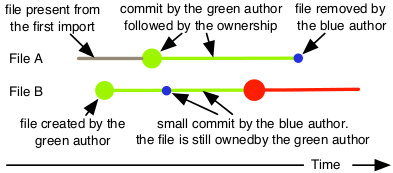
\includegraphics[width=0.5\textwidth]{./resources/girba2005.png}~
\caption{commit map}
\label{fig:commit_map}
\end{figure}

When this visualisation is applied to en entire, project, it becomes possible to detect behavioural pattern between developers. See annex[1].

\subsection{How Developers Develop Features}

In 2007 the same team published this paper, on a similar subject as the previous. This time, they focus is on the ownership of features, as well as files. The visualisation displays the ownership of files within the projects features, which are also structurally linked. The following image is a representation of this visualisation on a program that is designed to manage a mobile phone:\\
\\
\begin{figure}[p]
\centering
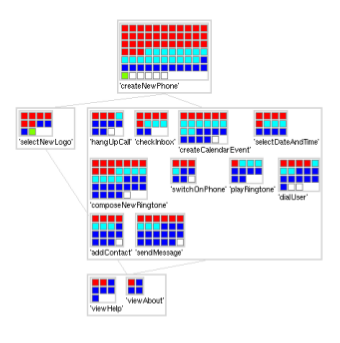
\includegraphics[width=0.4\textwidth]{./resources/girba2007.png}~
\caption{Ownership map By Feature}
\label{fig:ownership_map_by_feature}
\end{figure}

This visualisation makes it possible to determine who one might ask in order to help resolve a bug in a feature, rather than having to identify which file belong to which feature as one would need to do with the previous paper's visualisation[cite annex1].

\subsection{Dual Ecological Mesures in software development}





\end{document}
 
